\documentclass{bmcart}

%%%%%%%%%%%%%%%%%%%%%%%%%%%%%%%%%%%%%%%%%%%%%%
%%                                          %%
%% CARGA DE PAQUETES DE LATEX               %%
%%                                          %%
%%%%%%%%%%%%%%%%%%%%%%%%%%%%%%%%%%%%%%%%%%%%%%

%%% Load packages
\usepackage{amsthm,amsmath}
\usepackage{graphicx}
%\RequirePackage[numbers]{natbib}
%\RequirePackage{hyperref}
\usepackage[utf8]{inputenc} %unicode support
%\usepackage[applemac]{inputenc} %applemac support if unicode package fails
%\usepackage[latin1]{inputenc} %UNIX support if unicode package fails
\usepackage[spanish]{babel}


%%%%%%%%%%%%%%%%%%%%%%%%%%%%%%%%%%%%%%%%%%%%%%
%%                                          %%
%% COMIENZO DEL DOCUMENTO                   %%
%%                                          %%
%%%%%%%%%%%%%%%%%%%%%%%%%%%%%%%%%%%%%%%%%%%%%%

\begin{document}

	\begin{frontmatter}
	
		\begin{fmbox}
			\dochead{Research}
			
			%%%%%%%%%%%%%%%%%%%%%%%%%%%%%%%%%%%%%%%%%%%%%%
			%% INTRODUCIR TITULO PROYECTO               %%
			%%%%%%%%%%%%%%%%%%%%%%%%%%%%%%%%%%%%%%%%%%%%%%
			
			\title{Tiroiditis}
			
			%%%%%%%%%%%%%%%%%%%%%%%%%%%%%%%%%%%%%%%%%%%%%%
			%% AUTORES. METER UNA ENTRADA AUTHOR        %%
			%% POR PERSONA                              %%
			%%%%%%%%%%%%%%%%%%%%%%%%%%%%%%%%%%%%%%%%%%%%%%
			
			\author[
			  addressref={aff1},                   % ESTA LINEA SE COPIA IGUAL PARA CADA AUTOR
			  corref={aff1},                       % ESTA LINEA SOLO DEBE TENERLA EL COORDINADOR DEL GRUPO
			  email={jane.e.doe@cambridge.co.uk}   % VUESTRO CORREO ACTIVO
			]{\inits{A.D}\fnm{Alejandro} \snm{Domínguez Recio}} % inits: INICIALES DE AUTOR, fnm: NOMBRE DE AUTOR, snm: APELLIDOS DE AUTOR
		
			\author[
			  addressref={aff1},                   % ESTA LINEA SE COPIA IGUAL PARA CADA AUTOR
			  email={rafatravil@gmail.com}   % VUESTRO CORREO ACTIVO
			]{\inits{R.T}\fnm{Rafael} \snm{Trapero Vílchez}} % inits: INICIALES DE AUTOR, fnm: NOMBRE DE AUTOR, snm: APELLIDOS DE AUTOR
		
			
			%%%%%%%%%%%%%%%%%%%%%%%%%%%%%%%%%%%%%%%%%%%%%%
			%% AFILIACION. NO TOCAR                     %%
			%%%%%%%%%%%%%%%%%%%%%%%%%%%%%%%%%%%%%%%%%%%%%%
			
			\address[id=aff1]{%                           % unique id
			  \orgdiv{ETSI Informática},             % department, if any
			  \orgname{Universidad de Málaga},          % university, etc
			  \city{Málaga},                              % city
			  \cny{España}                                    % country
			}
		
		\end{fmbox}% comment this for two column layout
		
		\begin{abstractbox}
		
			\begin{abstract} % abstract
			
			%%%%%%%%%%%%%%%%%%%%%%%%%%%%%%%%%%%%%%%%%%%%%%%
			%% RESUMEN BREVE DE NO MAS DE 100 PALABRAS   %%
			%%%%%%%%%%%%%%%%%%%%%%%%%%%%%%%%%%%%%%%%%%%%%%%	
			
			\end{abstract}
			
			%%%%%%%%%%%%%%%%%%%%%%%%%%%%%%%%%%%%%%%%%%%%%%
			%% PALABRAS CLAVE DEL PROYECTO              %%
			%%%%%%%%%%%%%%%%%%%%%%%%%%%%%%%%%%%%%%%%%%%%%%
			
			\begin{keyword}
			\kwd{sample}
			\kwd{article}
			\kwd{author}
			\end{keyword}
		
		
		\end{abstractbox}
	
	\end{frontmatter}
	

	\section{Introducción}

\hrule
\vspace{5mm}
\\
La tiroides es una glándula pequeña situada en la parte anterior del cuello, encargada de la producción de dos hormonas tiroideas: la tiroxina (T4), que 
<<<<<<< HEAD
corresponde al 93 por ciento de hormona secretada por la glándula tiroides, y la 3,5,3-triyodotironina (T3) \cite{Stegmann} . Dicha glándula regula procesos metabólicos esenciales, tanto en la etapa de desarrollo, como en la edad adulta. Estos procesos están relacionados con el metabolismo energético, incrementando el consumo calórico, regulando el crecimiento y maduración de los tejidos y el recambio de prácticamente todos los sustratos, vitaminas y hormonas.  \cite{Stegmann} 
\\ \\
El término tiroiditis (HP:0100646) se asocia con todas aquellas enfermedades que presentan inflamación de la glándula tiroides \cite{Sweeney2014}. Los síntomas que produce la tiroiditis varían dependiendo de la enfermedad tiroidea que la produzca. No obstante, podemos diferenciar dos efectos diferenciados provocados por la tiroiditis \cite{Pulgarin} : 
=======
corresponde al 93 por ciento de hormona secretada por la glándula tiroides, y la 3,5,3-triyodotironina (T3) \cite{Stegmann} . Esta regula procesos metabólicos esenciales tanto en la etapa de desarrollo como en la edad adulta. \cite{Stegmann} 
\\ \\
El término tiroiditis (HP:0100646) se asocia con todas aquellas enfermedades que presenten inflamación de la glándula tiroides \cite{Sweeney2014}. Los síntomas que produce la tiroiditis variarán dependiendo de la enfermedad tiroidea que la produzca. No obstante, podemos diferenciar dos efectos diferenciados provocados por la tiroiditis \cite{Pulgarin} : 
>>>>>>> af19c8c0bd0178706be517ccd733e33c981467ab
\begin{itemize}
    \item Hipotiroidismo. Condición en la cual la glándula tiroides no puede producir la suficiente cantidad de hormonas tiroideas necesarias para cumplir con el requerimiento tisular.
    \item Hipertiroidismo. Incremento sostenido de las hormonas tiroideas debido al aumento de biosíntesis y secreción de la tiroides.
\end{itemize} 
\\ \\
<<<<<<< HEAD
\vspace{5mm}
Entre las enfermedades más conocidas que presenten tiroiditis tenemos la enfermedad de Hashimoto 'HT' (HP:0000872). Siendo la característica más común una elevación de los anticuerpos autoinmunes TPOAb y TGAb en las celulas tiroideas. HT estando presente aproximadamente en el 5 por ciento de la población mundial, siendo actualmente la enfermedad autoinmune con mayor incidencia \cite{Zheng2020}. Principalmente su sintomatología es bocio no-doloroso, hipotiroidismo y elevación de TPO \cite{Sweeney2014}. A su vez, encontramos una alta comorbilidad de HT con la diabetes tipo 1, Turner syndrome, Addison disease, y hepatitis C no tratada.\cite{Sweeney2014} 
Existen otros subtipos menos comunes de la tiroiditis, tales como tiroiditis infecciosa, tiroiditis post-parto o tiroiditis inducida por radiación. \cite{Sweeney2014}  
\vspace{20mm}

\\ \\
Diversos factores  intervienen en el desarrollo de enfermedades relacionadas con la tiroiditis: factores genéticos, factores ambientales (infecciones producidas por agentes externos), dietéticos (relacionados con los niveles de ingesta de yodo) o de otro tipo como el estrés, el tabaquismo o incluso el embarazo. Destacan los genéticos, siendo los de mayor implicación en este tipo de enfermedades. \cite{Hiromatsu}
\\ \\ 
Hasta la fecha se han encotrado un total de 46 genes asociados a la tiroiditis \cite{StringHP:0100646}. Aquellos genes con mas relaciones registradas son: el HLA-DR, los genes inmunorreguladores (CD40, CTLA-4, PTPN22, FOXP3 y CD25) y los genes específicos del tiroides (tiroglobulina [TG] y receptor de la hormona tiroestimulante [TSH]).
Estos, principalmente, están relacionados con dos procesos moleculares: la unión de proteínas y péptidos y con la actividad de los receptores inmunes. \cite{Hiromatsu}
\\ \\
En relación a los genes implicados en la unión de proteínas y péptidos; se encuentran involucrados en la regulación de citoquinas (SOCS1) y en el crecimiento celular, así como en la  apoptosis (PIK3CA) y en la supervivencia celular inducida por daño al ADN (PRKCD). Estando estos procesos inmiscuídos tanto en la propia fisiología de la tiroiditis, como en enfermedades autoinmunes o cáncer.\cite{StringHP:0100646, Yamada2022, PRKCDGeneCards}
\\ \\ 
Entre los genes asociados a la actividad de los receptores inmunes (actividad involucrada en el inicio de la respuesta inmune a partir de la recepción y transmisión de señales entre células) encontramos: IL2RG, IL7R, IL2RA, HLA-DQB1 y HLA-DQA1. Destacan la familia HLA  perteneciente al complejo MHC (Major histocompatibility complex), ya que juegan un papel fundamental en el sistema inmunológico presentando péptidos de proteínas extracelulares. \cite{HLA}Así como la familia de ILR, compuesta por IL2RG, IL7R y IL2RA. Estos genes son los responsables de la producción de receptores de citoquinas, participando en la regulación de la tolerancia inmune mediante el control de células T. \cite{StringHP:0100646}
\\ \\ \newpage
En la siguiente imagen podemos ver la red de genes relacionados con el fenotipo tiroiditis (HP:0100646), siendo representados de azul aquellos que intervienen en la actividad de los receptores inmunes, de rojo los que intervienen en la unión de péptidos y bicolor los que intervienen en ambas.
\vspace{5mm}
=======
Entre las enfermedades más conocidas que presenten tiroiditis tenemos la enfermedad de Hashimoto (HT). Es conocido que alredeor del 20-30 por ciento de la población sufre de HT. \cite{Zheng2020}. Principalmente la sintomatologia de HT es bocio-no doloroso, hipotiroidismo y elevación de TPO \cite{Sweeney2014}. A su vez existen otros subtipos tales como tiroiditis infecciosa, tiroiditis post-parto o tiroiditis inducida por radiación. \cite{Sweeney2014}
\\ \\
 Diversos factores  intervienen en el desarrollo de estas enfermerdades, como por ejemplo los factores de tipo ambiental (infecciones producidas por agentes externos), factores dietéticos (relacionados con los niveles de ingesta de yodo) u otro tipo de factores como el estrés, el tabaquismo o incluso el embarazo. \cite{Hiromatsu}
\\  \\ 
 Por ejemplo, hablando de la enfermedad de Hashimoto, el 50 por ciento de los factores que producen dicha enfermedad son genéticos, por lo que nos encontramos ante aquellos factores de mayor implicación. Siendo la característica más común, una elevación de los anticuerpos autoinmunes TPOAb y TGAb en las celulas tiroideas.\cite{Zheng2020} A su vez se ha encontrado una alta coexistencia de HT con la diabetes tipo 1, Turner syndrome, Addison disease, and  hepatitis C no tratada.\cite{Sweeney2014}
\\ \newpage
Hasta la fecha varios genes se han asociado al fenotipo, como el HLA-DR, los genes inmunorreguladores (CD40, CTLA-4, PTPN22, FOXP3 y CD25) y genes específicos del tiroides (tiroglobulina [TG] y receptor de la hormona tiroestimulante [TSH]), siendo estos son los más citados; no obstante, encontramos un total de 46 genes asociados al fenotipo. 
\\ \\
Estos genes principalmene están relacionados con dos procesos moleculares: la unión de proteínas y péptidos (importante en la estructura del cromosoma) y en la actividad de los receptores inmunes. Dicha actividad consiste en recibir señales y transmitirlas a células para iniciar una respuesta inmune en éstas.
\cite{Hiromatsu}
En la actividad de los receptores inmunes, están implicados los genes IL2RG, IL7R, IL2RA, HLA-DQB1 y HLA-DQA1. Podemos destacar estos dos últimos, siendo ambos pertenecientes a la clase MHC (Major histocompatibility complex). Ambos genes juegan un papel fundamental en el sistema inmune ya que presentan aquellos péptidos de proteínas extracelulares. \cite{HLA} 
\\ \\
Sin embargo,los genes restantes no se encargan de la unión de proteínas, pues encontramos varios que no participan en ninguno de los dos procesos moleculares. Destacar que  la familia de ILR, compuesta por IL2RG, IL7R y IL2RA , participan en ambos procesos, por lo que podemos afirmar que son de gran importancia en la tiroiditis. 

En la siguiente imagen podemos ver la red de genes relacionados con nuestro fenotipo, siendo representados de azul aquellos que intervienen en la actividad de los receptores inmunes, de rojo los que intervienen en la unión de péptidos y bicolor los que intervienen en ambas.
>>>>>>> af19c8c0bd0178706be517ccd733e33c981467ab
\begin{center}
 
    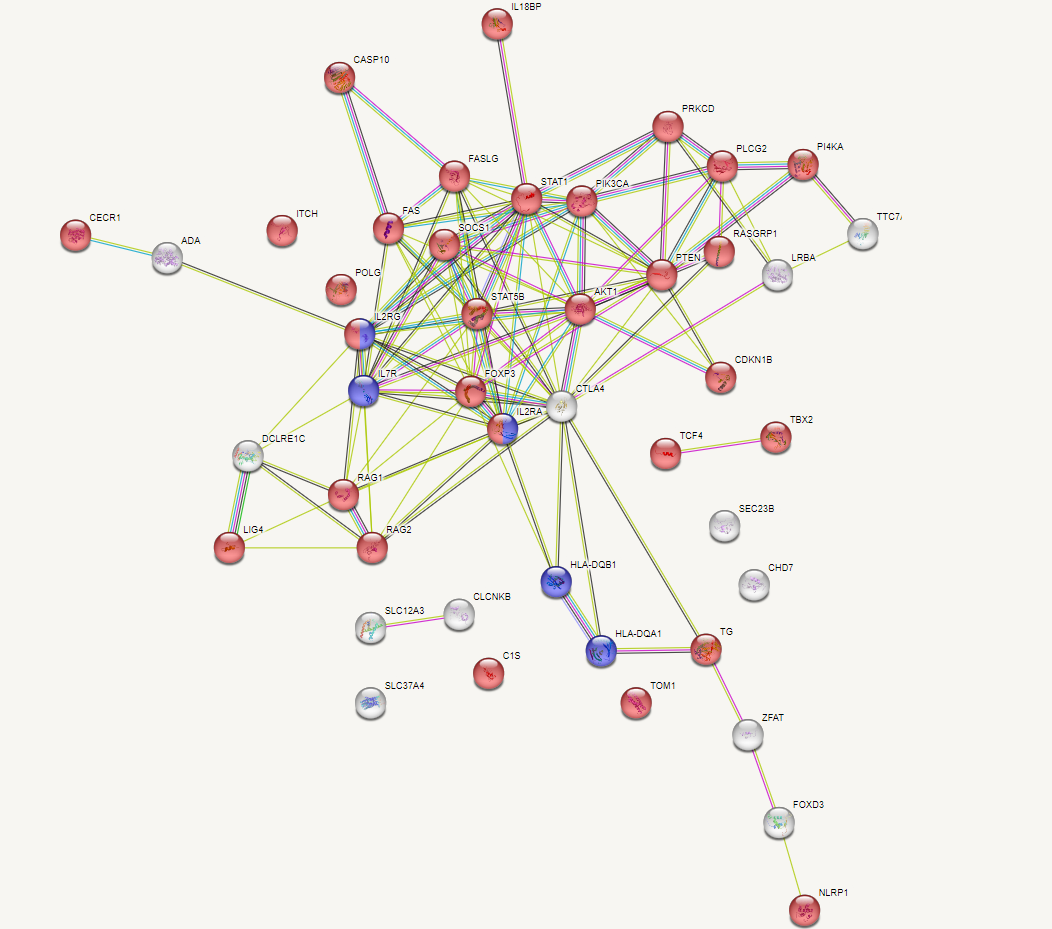
\includegraphics[scale=0.4]{figures/red de genes.png}
    
<<<<<<< HEAD
    Figure 2.1. Red de Genes HP:0100646
\end{center}
\\ \\ 
\vspace{5mm}
Los factores genéticos constan de una gran importancia en las enfermedades relacionadas con la tiroiditis, aunque en HT tienen especial relevancia, estando asociados al origen del 50 por ciento de los casos.\cite{Zheng2020} Encontramos 17 genes asociados a la enfermedad de Hashimoto. Algunos de estos genes (PTEN, PLCG2, CTLA4, TTC7A) se han encontrado involucrados en la enfermedad inflamatoria intestinal, con fisiología autoinmune. No obstante, existe una carencia de información sobre los procesos moleculares y las relaciones entre los genes involucrados en HT. Siendo estas mayormente obtenidas a partir de textmining sobre estudios de enfermedades no tiroideas con fisiología autoinmune. \cite{StringHP:0000872}
\\ \\  
Dada la importancia de los factores genéticos en la tiroiditis y del gap de conocimiento identificado en HT, el estudio se centra en la realización de un análisis de los diferentes genes asociados a dichos fenotipos y de las funciones moleculares en los que estan asociados. Para la identificación de nuevas relaciones genéticas y procesos moleculares asociados se tiene en cuenta el tipo de interacción (física, co-expresión, databases, etc...) entre los genes involucrados, así como las funciones moleculares compartidas por ambos.





=======
    Figure 2.1. Red de Genes
\end{center}
\\ \\
Dada la importancia de los factores genéticos en este fenotipo (HP:0100646), el estudio se centrará en la realización de un análisis de los diferentes genes asociados a dicho fenotipo y de las relaciones funcionales entre estos. 
\\ \\  \newpage 
Se tendrán en cuenta el tipo de interacción (física, co-expresión, databases, etc...) a partir de las cuales diluciar los diferentes clusters. Estos clusters ayudarán a clasificar genes en base a la función molecular que desempeñen. La distribución de genes resultante ayudará a descubrir cuales de ellos tienen una mayor relevancia.
\\ \\
>>>>>>> af19c8c0bd0178706be517ccd733e33c981467ab





	\section{Materiales y métodos}
\subsection*{Datos fenotipos}
El conjunto inicial de interacciones gen-gen asociados a los fenotipos HP:0100646 Thyroiditis y HP:0000872 Hashimoto fue obtenido a partir de la base de datos STRING (https://string-db.org/). La base de datos STRING  integra conocimiento sobre las relaciones entre proteínas, incluyendo desde interacciones físicas hasta relaciones funcionales. Las relaciones son determinas a partir de una serie de evidencias con una significancia asociada. \cite{Szklarczyk2021}  Las evidencias que determinaron las redes de interacción de nuestros fenotipos son las siguientes: (1) textmining, (2) experimentos, (3) bases de datos, (4) co-expresión, (5) vecindad, (6) fusión de genes, (7) co-ocurrencia. La significancia mínima asociada a cada interacción determinada fue de 0.7. Encontramos un total de 46 genes asociados al fenotipo  HP: 0100646 Thyroiditis y 17 a  HP:0000872 Hashimoto. 
\subsection*{Propagación de red}
Realizamos una propagación de red al conjunto de genes incial asociado a cada fenotipo. Añadimos un total de 200 genes a los conjuntos de genes iniciales.
\subsection*{Enriquecimiento funcional}
El enriquecimiento funcional es crucial en la interpretación de datos ómicos. Realizamos un enriquecimiento funcional KEGG a las comunidades presentes en las redes asociadas a cada fenotipo. Asignamos a cada comunidad la función molecular correspondiente en base al gene ratio obtenido en el enriquecimiento. Fijamos el umbral del p-value en 0.05. \\ 
La Kyoto Enciclopedia de Genes y Genomas (KEGG) es una base de datos aplicada al entendimiento de la información funcional en organismos a partir de su información genética. La base de datos KEGG fué desarollada por los laboratorios Kanehisa en 1995 y actualmente es un referente en la integración y interpretación de datos moleculares generados por secuenciación  genómica u otras tecnologías de alto rendimiento. \\ 
La información se encuentra agrupada en cuatro bloques según su sentido biológico: genes y proteínas (información genómica), sustancias químicas (información química), relaciones de redes (información de sistema), enfermedad y drogas asociadas (información sanitaria). El mayor componente de información se denomina PATHWAY y consiste en diagramas asociados a rutas moleculares, incluyendo rutas metabólicas y regulativas. \\
La información en KEGG esta representada en forma de grafo y técnicas computacionales son aplicadas para detectar relaciones entre las características del grafo y funciones celulares anotadas.  \\
Mapeando genes en el genoma y productos en las rutas moleculares, KEGG predice interacciones entre redes y funciones celulares asociadas. Los genes del genoma son representados como nodos conectados en una dimensión y las rutas moleculares es un grafo de productos de lo genes con un patrón de conexiones mas complejo. \cite{Ogata1999, Minoru}\\
Para el acceso y mapeo de los genes de nuestro experimento en KEGG, utilizaremos el paquete R clusterProfiler.Cluster profiler fue publicado en 2012 y diseñado para realizar análisis de sobrerepresentación usando términos GO y KEGG. Actualmente soporta varias ontologías y anotaciones de pathways, y tiene miles de especies con capacidad de anotación. A través de una pequeña interfaz permite la manipulación y visualización de los resultados de enriquecimientos. Complementando las funcionalidades de clusterProfiler se han incorporado multitud de paquetes. Entre estos GoSemSim para eliminar términos GO redundantes, o enrichPlot para visualizar los resultados del enriquecimiento \cite{Wu2021}.
\subsection*{Búsuqueda de funciones comunes}
\subsection*{Análisis de comunidades}
	
\section{Resultados}

	\section{Discusión}
A raíz de los resultados obtenidos en la comparación de clusters, se ha determinado que hay 3 pathways donde clusters de ambos fenotipos participan: 'JAK-STAT signaling pathway', 'Alzheimer disease' y 'Bacterial invasion of epithelial cells'.Los clusters asociados a cada fenotipo en los pathways 'Bacterial invasion of epithelial cells' y 'Alzheimer disease' son los mismos. No osbtante, el gene ratio asociado al pathway 'Alzheimer disease' (0.1347), es mayor que el asociado a 'Bacterial invasion of epithelial cells' (0.1088). Por esto último descartaremos para el análisis el pathway 'Bacterial invasion of epithelial cells'.
\\ \\
Para el primer pathway los genes 'IL2RG' y 'JAK3' están presentes en el cluster de Hashimoto, así como en el de Tiroiditis. No obstante, unicamente "IL2RG" pertenece al conjunto de genes semilla. Para el segundo pathway solo encontramos un gen que esté en ambos fenotipos, el 'PIK3R2', el cual pertenece a los genes obtenidos a partir de la propagación de red. Se añade que, además, hay indicidios de  interacción física entre los genes 'IL2RG', 'JAK3' y 'PIK3R2' (R-HSA-1295544). Además dichos genes están asociados a la producción de IL-4, citoquina involucrada en procesos de regulación inmunitaria\cite{Gadani2012}. 
\\ \\
Uno de los objetivos del proyecto, y a modo de líneas futuras, era intentar expandir la red de genes de Hashimoto a partir de genes pertenecientes a la de Tiroiditis. Anteriormente hemos explicado que existen 3 genes que se encuentran en clusters de ambos fenotipos. Pero para este caso, nos interesan aquellos que están presentes en Tiroiditis pero no en Hashimoto. Unos posibles candidatos serían, basándonos en el pathway de 'vía de señalización JAK-STAT' , los genes 'IL2RB', 'EPOR','IL10RA', 'PDGFRA','PDGFRB','IL12RB2','IL27RA','IFNAR1','IL22RA1',
'EGFR','IL10RB','IFNGR2' y 'IL7R'. Basándonos en el segundo patwhay 'Alzheimer disease', encontramos los siguientes genes candidatos: 'PI4KA', 'PIK3R3' y 'PIK3R1'.
\\ \\
Recalcar que todos estos genes son candidatos y sería necesario un análisis posterior para poder determinar más relaciones de estos genes con los ya presentes en la red de genes de Hashimoto.


	\section{Conclusiones}
Tras una comparación de las redes genéticas de Tiroiditis y Hashimoto, finalmente hemos obtenido varios genes candidatos para la expansión de la red de Hashimoto.
El análisis bioinformático realizado ha consistido en varios pasos.El primero fue una expansión de ambas redes hasta obtener 200 genes en total. El siguiente paso fue la agrupación de estos genes en comunidades para su posterior análisis funcional.
Una vez las comunidades estaban asociadas a un pathway biológico, el paso final fue comparar (para ambos fenotipos) que pathways comunes compartían y, a partir de las comunidades asociadas a estos, poder determinar genes pertenecientes a la red de Tiroiditis que pudieran formar parte de la de Hashimoto.

Con estos genes candidatos se pueden realizar análisis posteriores y una investigación biológica más exhaustiva para poder decidir si realmente pueden formar parte de la red de Hashimoto.

A parte de determinar varios genes candidatos  hemos obtenido otros resultados interesantes. Por ejemplo, una relación de la tiroiditis con la enfermedad de Alzheimer. 





	
	
	%%%%%%%%%%%%%%%%%%%%%%%%%%%%%%%%%%%%%%%%%%%%%%
	%% OTRA INFORMACIÓN                         %%
	%%%%%%%%%%%%%%%%%%%%%%%%%%%%%%%%%%%%%%%%%%%%%%
	
	\begin{backmatter}
	
		\section*{Abreviaciones}%% if any
			HT: Enfermedad de Hashimoto
		
		\section*{Disponibilidad de datos y materiales}%% if any
			https://github.com/GitHubAlejandroDR/project-systems-biology
		
		\section*{Contribución de los autores}
			Usando las iniciales que habéis definido al comienzo del documento, debeis indicar la contribución al proyecto en el estilo:
			J.E : Encargado del análisis de coexpresión con R, escritura de resultados; J.R.S : modelado de red con python y automatizado del código, escritura de métodos; ...
			OJO: que sea realista con los registros que hay en vuestros repositorios de github. 
		
		
		%%%%%%%%%%%%%%%%%%%%%%%%%%%%%%%%%%%%%%%%%%%%%%%%%%%%%%%%%%%%%%%%%%%%%%%%%%%%%%%%%%%%%%%%
		%% BIBLIOGRAFIA: no teneis que tocar nada, solo sustituir el archivo bibliography.bib %%
		%% por el que hayais generado vosotros                                                %%
		%%%%%%%%%%%%%%%%%%%%%%%%%%%%%%%%%%%%%%%%%%%%%%%%%%%%%%%%%%%%%%%%%%%%%%%%%%%%%%%%%%%%%%%%
		
		\bibliographystyle{bmc-mathphys} % Style BST file (bmc-mathphys, vancouver, spbasic).
		\bibliography{bibliography}      % Bibliography file (usually '*.bib' )
	
	\end{backmatter}
\end{document}
